\chapter[Existing work - Sondovač]{Existing work - Sondovač}
\label{kap:existing_work}

In this chapter, we will take a closer look at the pipeline and the workflow of Sondovač. We 
will also specify the input and output data format and consider them from the informatic and 
more formal point of view. Finally, detailed description of the tools and software that are used by 
Sondovač will be listed. 

\section{Sondovač origins}

Sondovač is a Czech neologism standing for "Probe-maker". It was created by Roswitha Schmickl, 
Aaron Liston, Vojtěch Zeisek and others. 
Sondovač is an interactive and automated script to create orthologous low-copy nuclear 
probes for further use by the Hyb-Seq protocol. It uses transcriptome and genome skim data. 
Sondovač does not require strong bioinformatic skills nor high-performance computer. It is 
intended for either Linux or Mac OS X. 

\section{The workflow overview}

Sondovač is written in BASH, an Unix shell and a command language \cite{bash}. It has three 
parts: Sondovač\_part\_a.sh, the Geneious \cite{geneious} intermediate part and Sondovač\_part\_b.sh. Between 
the parts a and b of Sondovač it is necessary to manualy input the output from the part a into 
another software - Geneious, for data processing and then run the part b on the output from the software. 


\subsection{Sondovač part a}%Don't forget we already know here what type of data we have. No we don't

\subsection{The input and output data}

\subsection{Input data for part a}
Input data for part a of Sondovač consist of 5 files, 1 of them being optional. 
\begin{enumerate}
\item Transcriptome input file in FASTA format

The file consists of several blocks with same format: On the first line of a block there is a '>' character followed 
by an unique description of the sequence, in this case a number. On the next few lines, there is the actual sequence 
composed of 'A', 'C', 'G' or 'T' characters. 
\item Plastome reference sequence input file in FASTA format

This file is used in both parts. It consists of a single long sequence and the starting line with '>' and the sequence's 
unique description. 

\item Mitochondriome reference sequence input file in FASTA format (Optional)

The file contains a single sequence along with the first line describing it. It is optional, because the size of a plant
mitochondrial genome can vary greatly and have high rearrangement rates. 

\item Paired-end genome skim input file in FASTQ format (first file, the forward reads)

\item Paired-end genome skim input file in FASTQ format (second file, the reverse reads)

Other than the input files, Sondovač requires a minimum total locus length to be set. 

Output data from part a are the input files for Geneious. 

\subsection{Input data for part b}
Input data for part b of Sondovač consist of 3 files and include the output data from Geneious. 
\begin{enumerate}

\item Input file in TSV format (output of Geneious assembly)

\item Input file in FASTA format (output of Geneious assembly)

\item Plastome reference sequence input file in FASTA format

This file is used in both parts. It consists of a single long sequence and the starting line with '>' and the sequence's 
unique description. 
\end{enumerate}


\section{Workflow, pipeline}

The part a of the script covers 6 steps: 

\begin{enumerate}
\item Removing the transcripts that share $\geq$ 90\% sequence similarity

We want to get low-copy nuclear orthologous probes. To minimize the enrichment of multi-copy loci, the Sondovač script removes transcripts that 
are too similar; share $\geq$ 90\% sequence similarity. This is done using BLAT and UNIX commands. From this we get unique transcripts that we match against processed reads. 

\item Removing the reads of plastid origin

Since we want only nuclear probes, the raw paired-end genome data is stripped of the reads that have plastid origin, utilizing the reference input sequences. Tools used for 
this are Bowtie 2 and Samtools. 

\item Removing the reads of mitochondrial origin

In the same manner, the reads of mitochondrial origin are removed from the paired-end genome data, if the list of mitochondrial sequences is present. Bowtie 2 and Samtools are 
used. 

\item Combining the paired-end reads

Subsequently, the paired-end reads without plastid and mitochondrial reads are combined using FLASH. 

\item Matching the unique transcripts and the filtered, combined genome skim reads sharing $\geq$ 85\% sequence similarity. 

Sequences that are well-preserved and therefore present amongst several related species make good genetic markers. Since transcripts are 
the sequences that are translated into proteins, they rarely change their genetic composition, eg. the bases they consist of. The Sondovač 
script matches the unique transcripts with the processed paired-end genome skim data. Using BLAT and Unix commands, only sequences that have 
$\geq$ 85\% similarity are kept.  

\item Filtering the BLAT output

\begin{enumerate}
\item Choosing the transcript or genome skim sequences for further processing

Either transcript or genome sequences are used as the basic sequences for designing the probes. The choice depends on the phylogenetic depth that should be obtained, but it doesn't 
matter if the researched taxa are closely related. Defaultly, the genome skim data is used. 

\item Removing the transcripts with more than 1000 BLAT hits

While making an alignment, BLAT makes hits - short similar sequences. The transcripts that achieve $\geq$ 1000 BLAT hits while matching them with filtered 
combined genome skim reads are removed to avoid repetitive elements. Unix commands are used for filtering and the amount of hits can be adjusted; it can be an 
integer ranging from 100 to 10000. 

\item Removing the transcript or genome skim BLAT hits containing masked nucleotides

Hits that contain masked nucleotides (nucleotides that are unknown or have various options) are removed as well. 

\end{enumerate}
\end{enumerate}


\subsection{Geneious}

After filtering the BLAST output, de novo assembly of BLAT hits into larger contigs commences. This part is done by Geneious, a desktop software platform 
that can analyze, asslemble or align sequences. The user has to take output of Sondovač part a and manually process the data with Geneious using the medium 
sensitivity / fast setting. 

\subsection{Sondovač part b}
Sondovač part b covers 4 steps. The output data from Geneious assembly and the plastome reference are the input files for part b. 
  
\begin{enumerate}
\item Retention of those contigs that comprise exons greater or equal than bait length and have a certain total locus length

Sequences that are too short aren't good genetic markers, because it's more likely that their presence in the genome is coincidental. Thus, the script picks those contigs that 
comprise exons with a minimum bait length greater than 120 base pairs and have a set minimum total locus length (the recommended length is 600bp and it has to be a multiple of 
the bait length), although these values can be adjusted. The selection is done using Unix commands. 

\item Removal of probe sequences sharing greater or equal than 90\% sequence similarity

We don't want the probes to target multiple similar loci, so similar sequences or duplicates are removed using CD-HIT. 

\item Retention of those contigs that comprise exons greater or equal than bait length and have a certain total locus length

A second filtering for sequences that are too short commences. The parameters are the same as before. 

\item Removal of probe sequences sharing greater or equal than 90\% sequence similarity with the plastome reference

Lastly, the sequences that are present in the plastome reference are removed, since we want to ensure we are targeting only nuclear probes. This is done by BLAT and Unix commands and 
only sequences that have similarity $\geq$ 90\% are removed. 

\end{enumerate}

\subsection{Additional removal of plastid sequences}

If any remaining plastid sequences are detected, they have to be removed manually from the final output of part b of Sondovač script, since we preffer nuclear probes and 
plastid genes would occupy too much space on the Illumina lane during target enrichment. 

\end{enumerate}

\begin{figure}
\centerline{
	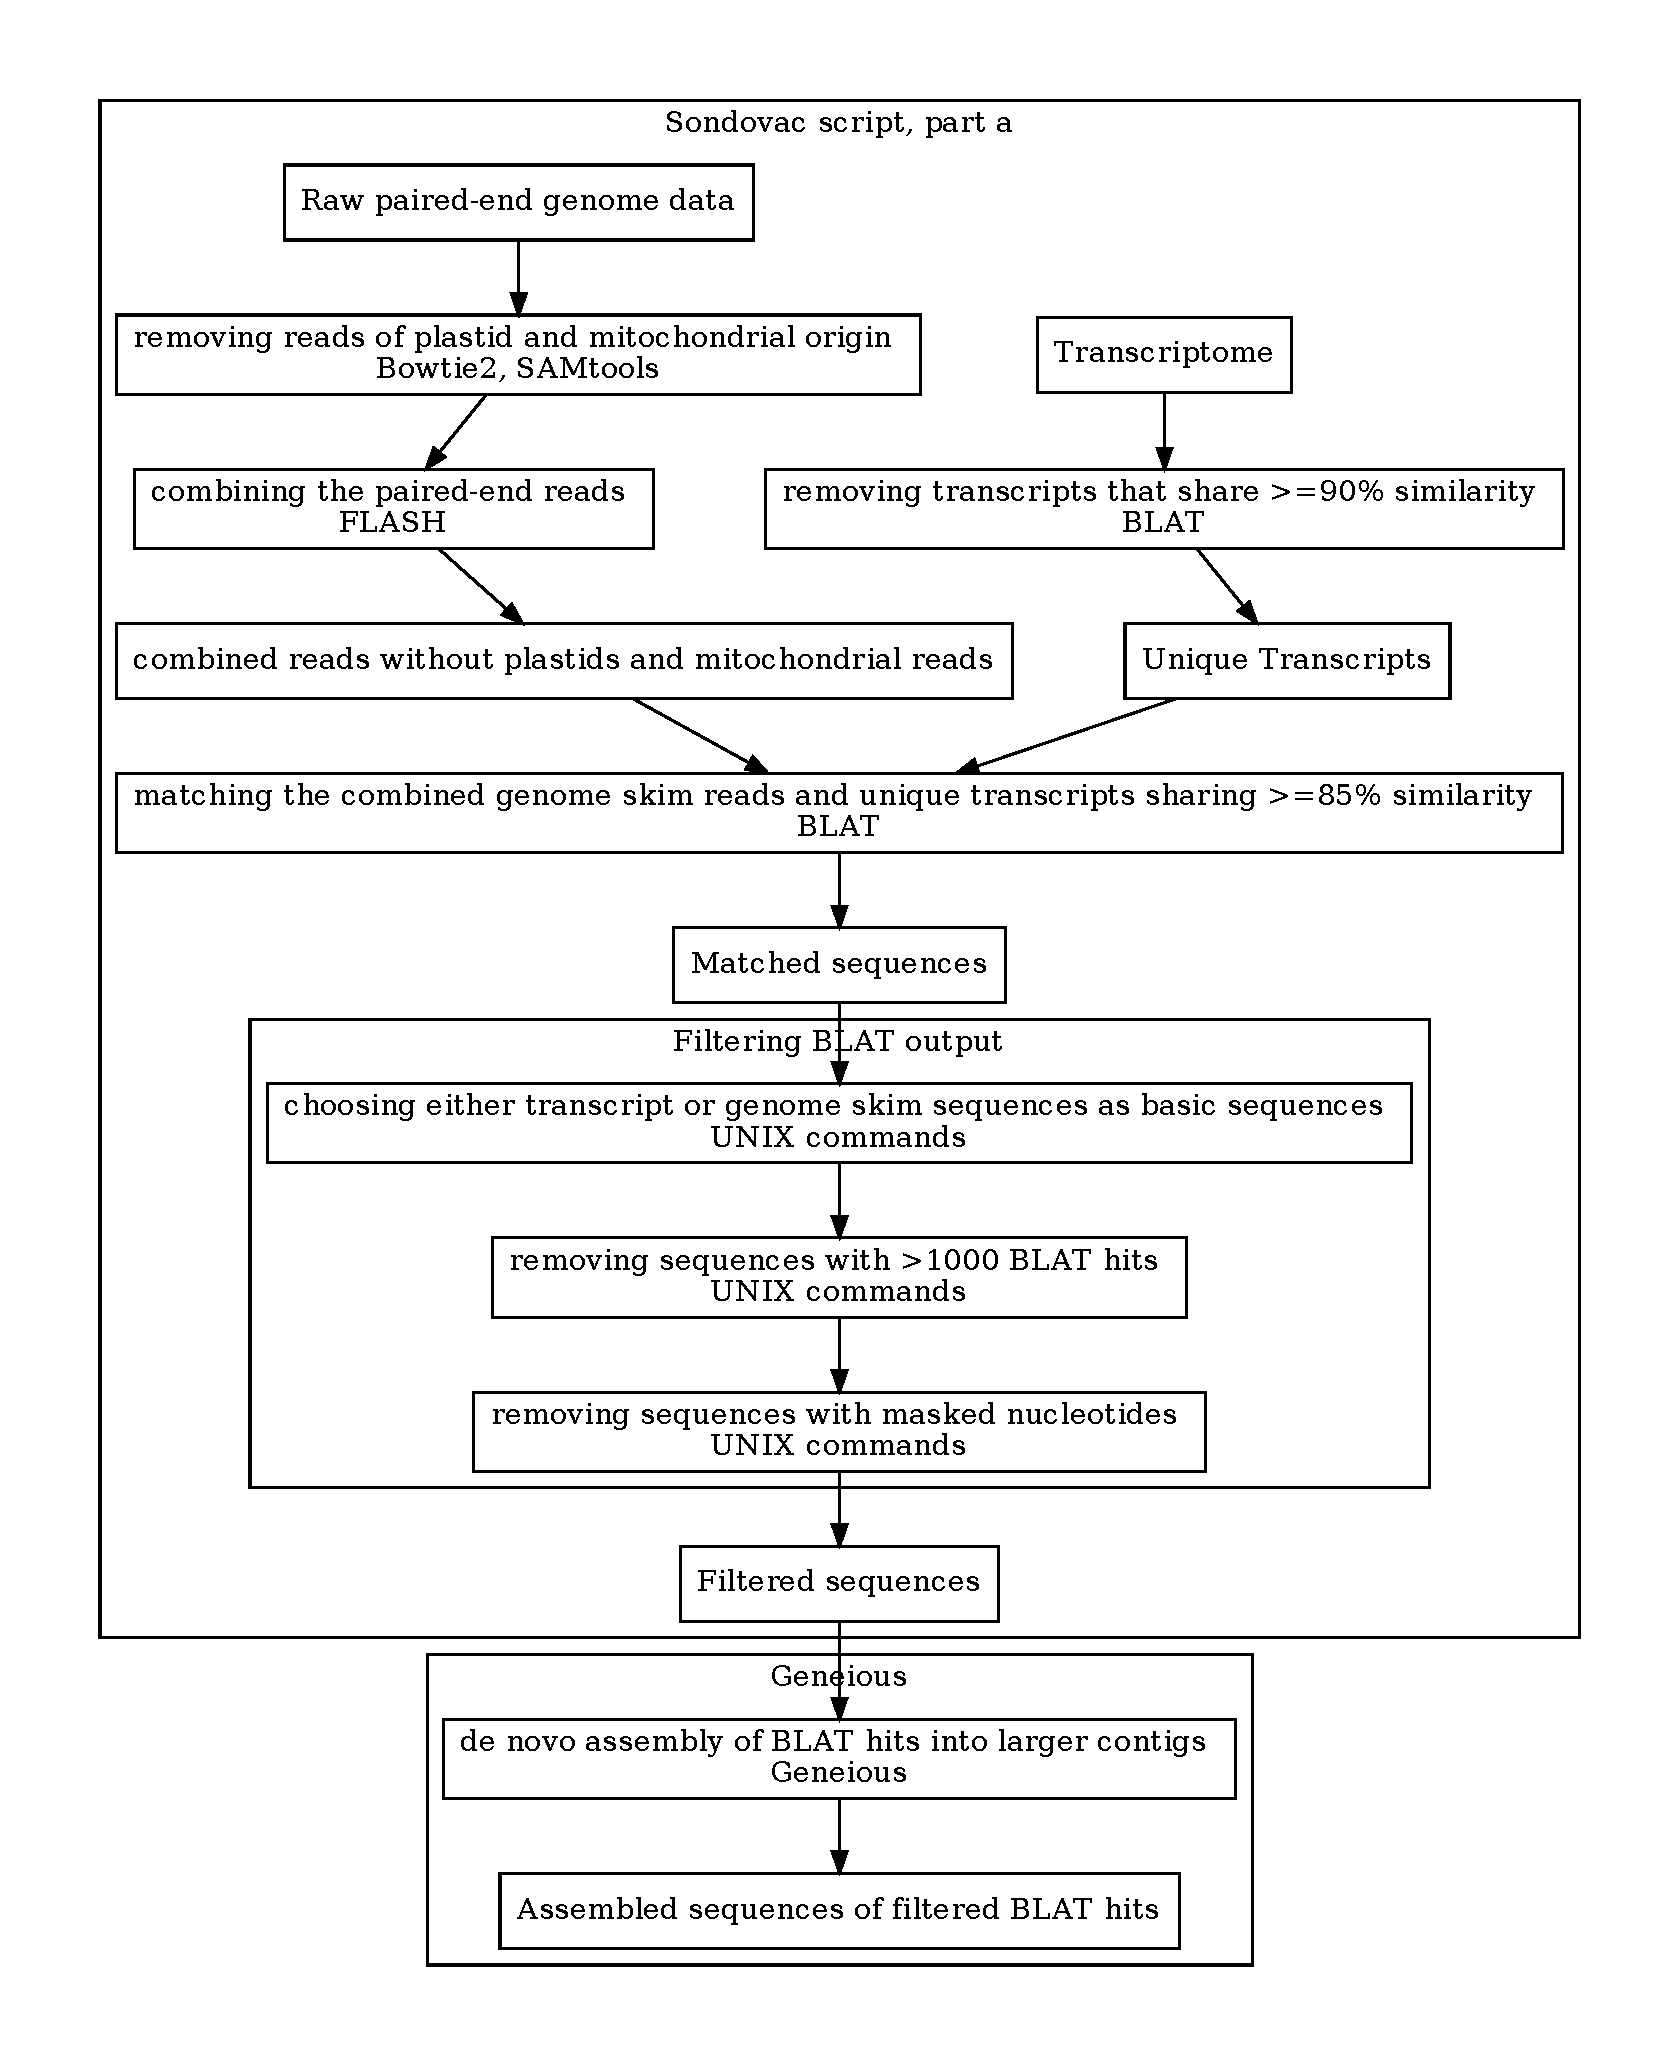
\includegraphics[width=1\textwidth]{graphs/sondovac_overview}
}
\caption[Sondovač pipeline workflow]{Flowchart illustrating the workflow of Sondovač script, part a and step with the Geneious software.}
\label{obr:workflowa}
\end{figure}

\begin{figure}
\centerline{
	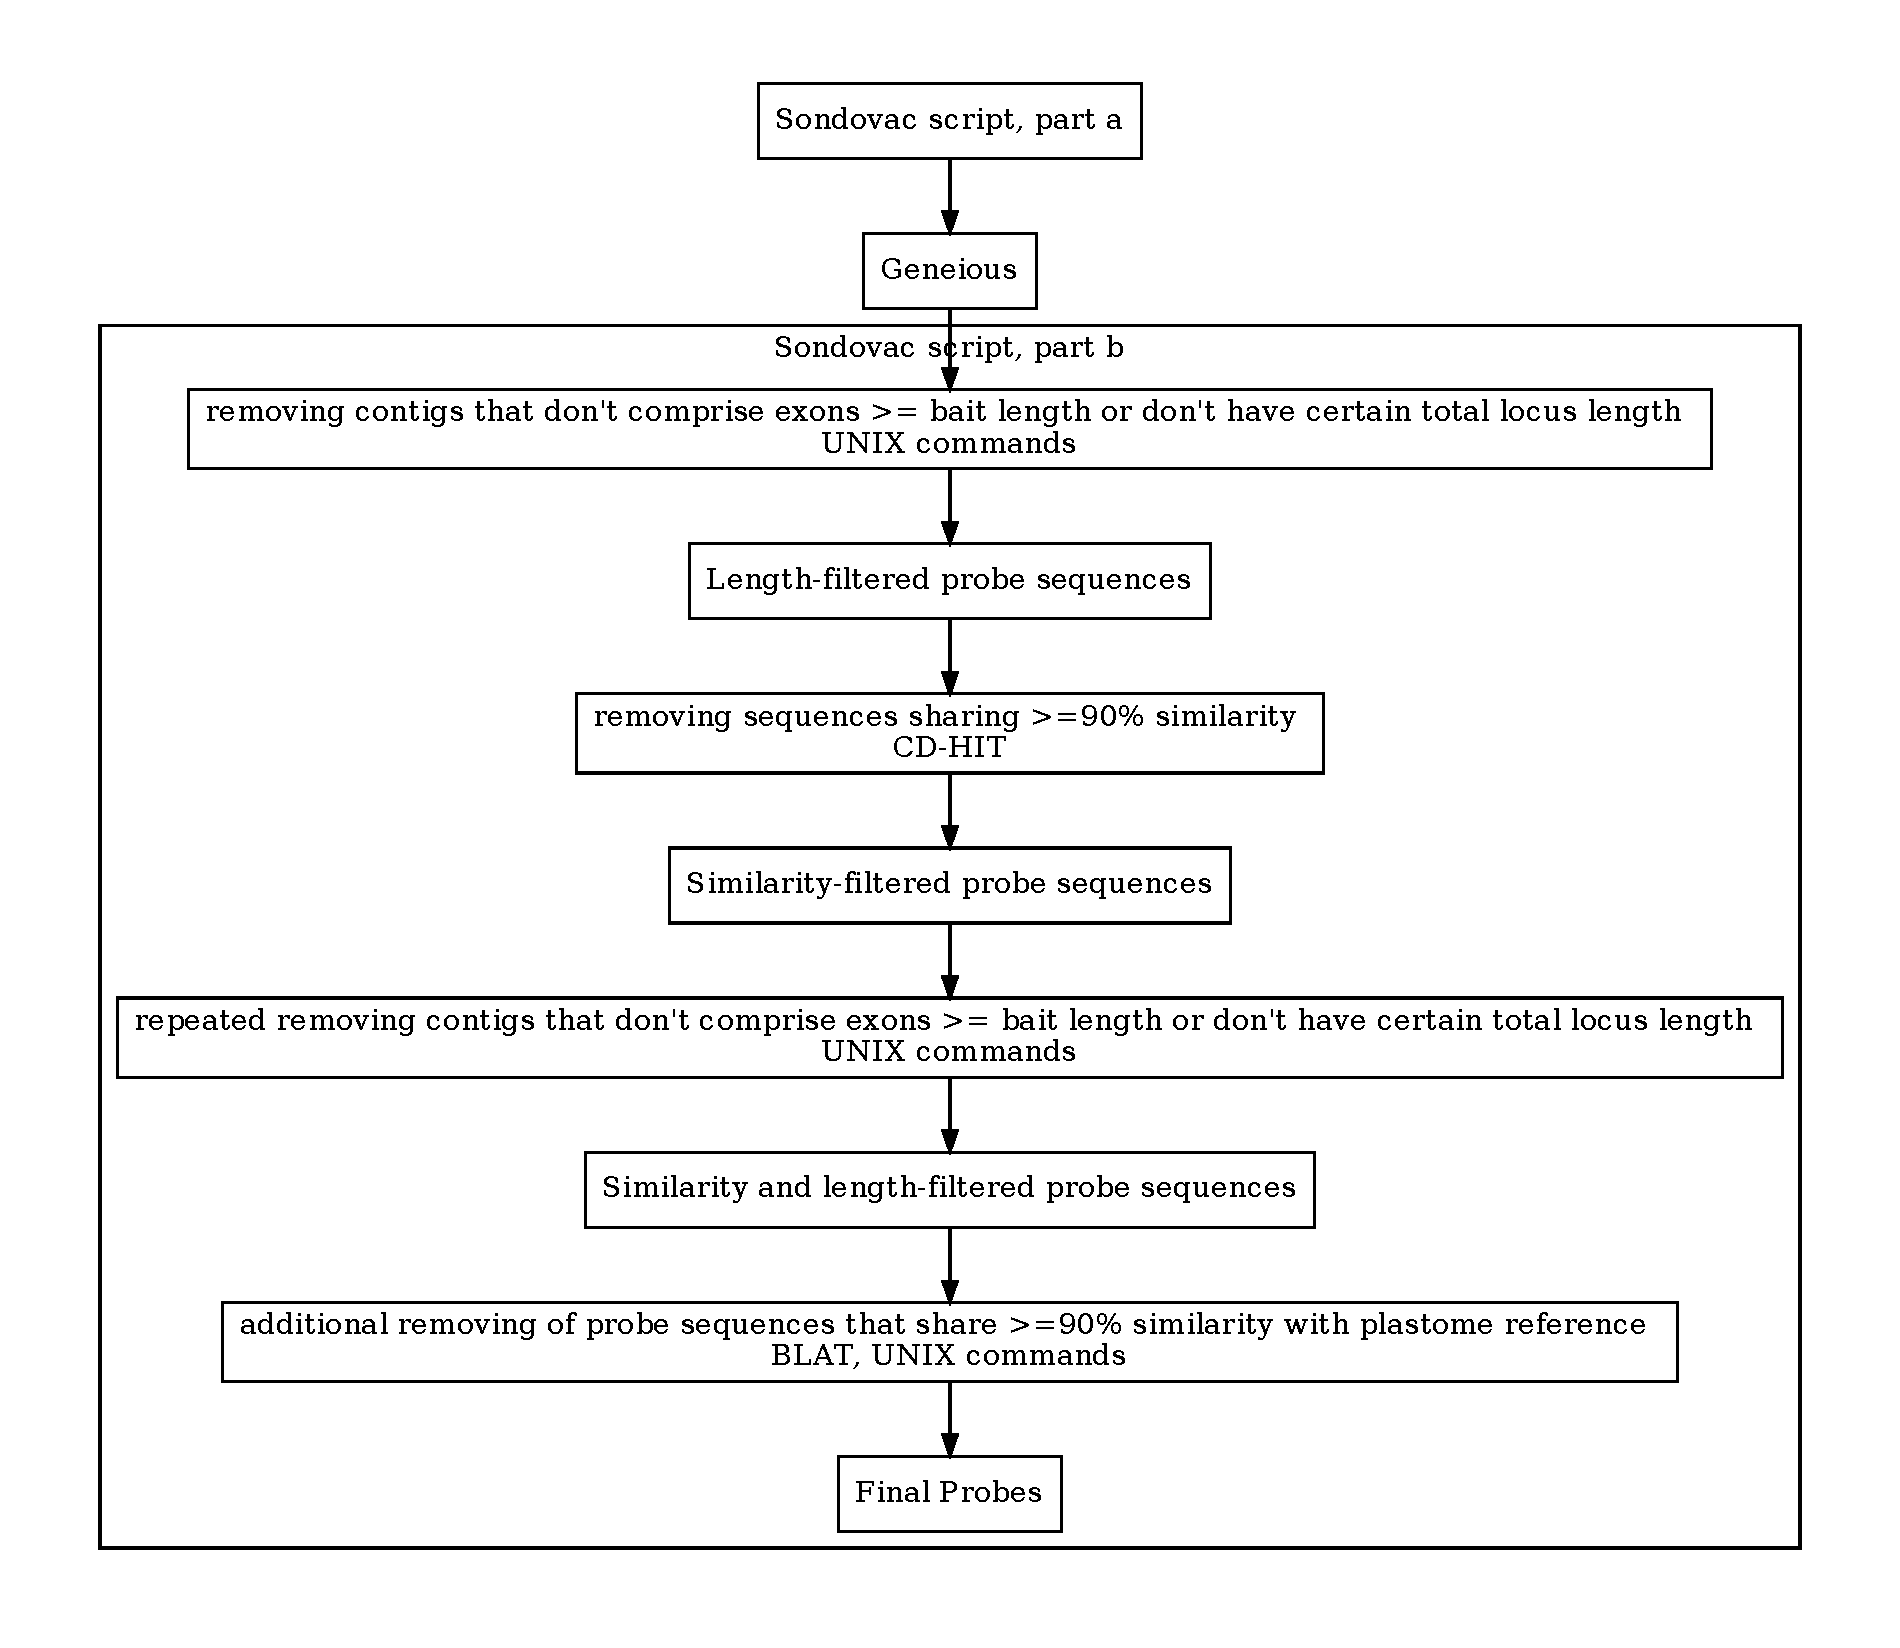
\includegraphics[width=1\textwidth]{graphs/sondovac_overview_part_b}
}
\caption[Sondovač pipeline workflow -- part b]{Flowchart illustrating the workflow of Sondovač script, part b.}
\label{obr:workflowb}
\end{figure}


\section{Output data}
Each part of the Sondovač pipeline has its own output data. Some of them are further used in the pipeline and other files are purely for user. In this section, we will 
take a look at the output data from various parts of the Sondovač script. 
An asterisk (\verb_*_) in the name of file indicates the part of the file name that is specified by the user with the '-o' flag. Default value is 'output'. 

\subsection{Output data - part a}

Only the last file is necessary for further processing as the input for Geneious. However, other files may be useful for the user. 
Sondovač, part a, creates the following files: 

\begin{enumerate}

\item \verb_*_\_renamed.fasta 

Copy of the transcriptome file where the labels of FASTA sequences were changed - unique numbers now correspond to the original file's line numbers. 

\item \verb_*_\_old\_and\_new\_names.tsv 

This file contains two columns - labels of the original sequences as it was in the transcriptome file provided by the user in the first, and new sequence labels in the 
second. This file and the \verb_*_\_renamed.fasta file can be used to trace back certain sequences or probes. 

\item \verb_*_\_blat\_unique\_transcripts.psl

Unique transcripts that are the output of BLAT after removal of the sequences that have $\geq$ 90\% similarity. 

\item \verb_*_\_unique\_transcripts.fasta

Unique transcripts that are the output of BLAT in FASTA format. 

\item \verb_*_\_genome\_skim\_data\_no\_cp\_reads

Genome skim data without the cpDNA reads - after the chloroplast DNA is removed. 

\item \verb_*_\_genome\_skim\_data\_no\_cp\_no\_mt\_reads

Genome skim data without the mtDNA reads - after the mitochondrial DNA is removed. This file is present only if the mitochondriome reference data was provided. 

\item \verb_*_\_combined\_reads\_co\_cp\_no\_mt\_reads

Paired-end genome skim reads that are combined. 

\item \verb_*_\_blat\_unique\_transcripts\_versus\_genome\_skim\_data.pslx

Output of BLAT after matching the unique transcripts and combined paired-end genome skim reads that have $\geq$ 85\% similarity. 

\item \verb_*_\_blat\_unique\_transcripts\_versus\_genome\_skim\_data.fasta

Output of BLAT after matching the unique transcripts and combined paired-end genome skim reads in FASTA format. 

\item \verb_*_\_blat\_unique\_transcripts\_versus\_genome\_skim\_data-no\_missing\_fin.fsa

Final sequences for further use in Geneious. This is a FASTA file and the only file that is used further in the pipeline. 


\end{enumerate}

\subsection{Output data - Geneious}

The output data from Geneious is the input data for the Sondovač script, part b, along with the plastome reference. 
Geneious output consists of two files: 
\begin{enumerate}
\item Assembled sequences from Geneious - a file exported in TSV format
\item Assembled sequences from Geneious - a file exporded in FASTA format
\end{enumerate}

\subsection{Output data - part b}

The Sondovač script, part b creates the following files: 

\begin{enumerate}
\item \verb_*_\_prelim\_probe\_seq.fasta

Preliminary probes in FASTA format. 

\item \verb_*_\_prelim\_probe\_seq\_cluster\_100.fasta

Unclustered exons and exons that have 100\% sequence identity - the bases match exactly between two different sequences. The file is in 
FASTA format. 

\item \verb_*_\_prelim\_probe\_seq\_cluster\_90.clstr

Unclustered exons and exons that have more than certain sequence identity in CLSTR format. 

\item \verb_*_\_unique\_prelim\_probe\_seq.fasta

Unclustered exons and exons that have less than a certain sequence similarity. 

\item \verb_*_\_similarity\_test.fasta

Contigs that comprise exons with greater or equal minimum bait length and have a certain minimum total locus length. 

\item \verb_*_\_target\_enrichment\_probe\_sequences\_with\_pt.fasta

Probes in FASTA format, that contain putative plastid sequences. If any BLAT hits were present, the possible plastid sequences are listed in the 
\verb_*_\_possible\_cp\_dna\_gene\_in\_probe\_set.pslx file. 

\item \verb_*_\_possible\_cp\_dna\_gene\_in\_probe\_set.pslx

A list of putative chloroplast sequences in case of any BLAT hits. These sequences are best to be removed from the final probe list, as we preffer nuclear probes. 

\item \verb_*_\_target\_enrichment\_probe\_sequences.fasta

The final list of probes in FASTA format. 

\end{enumerate}


\section{Used software and tools}
Sondovač uses a broad variety of tools and scientific software packages, both freeware and payware. It is mainly coded in BASH, but it also uses smaller python 
scripts. We will take a closer look at what each of the tools is and what it does in the Sondovač script. 

\subsection{Programming languages}
Here we will take a look at programming languages the Sondovač script uses. 
%What it is, what it is used for, citation, what part does it play in Sondovač

\begin{enumerate}
\item BASH

BASH is a command line interpreter (or shell) and a command language for Unix. It's a programming scripting language accessible through a terminal in 
any Unix-based operating system. It is a free software. Scripts written in BASH usually have the extension \verb_*_.sh. 

The Sondovač script is written in BASH. Using this language, it runs other programms and scripts. It is also used to work with files or manipulate and filter the data. 

\item Python

Python is an interpreted programming language. 
Several scripts that Sondovač uses are coded in Python. 

\end{enumerate}

\subsection{Tools and software}

In this section, we will list the most inportant tools and software that Sondovač uses. Some of the software changed or was replaced with a newer version of Sondovač, 
but the tools and software listed here comprise are essential part of Sondovač. 
Sondovač uses the following software: 

\begin{enumerate}

%\item Bam2fastq
%Dropped in favor of Samtools
%Picard is not used

\item BLAT

BLAT -- the BLAST like alignment tool -- is a pairwise sequence alignment algorithm. \cite{kent2002blat}
It is used by the Sondovač script to match reads to unique transcripts and for other alignments. It is used 
in both parts of the script. 

\item Bowtie2

Bowtie2 is a memory-efficient tool used for aligning sequencing reads to longer reference sequences. It keeps an FM index to save memory. Bowtie2 has 
local, gaped and paired-end alignment modes. \cite{bowtie2}
%We used Bowtie2 for aligning the sequences we need to keep to the sequences we have. 
It is used in Sondovač, part a to find plastome or mitochondrione sequences in the genome. 

\item CD-HIT

CD-HIT is a program for clustering and comparing protein or nucleotide sequences. It can compare two databases and identify sequences that 
are similar above a threshold. \cite{cd-hit}
It is used in Sondovač, part b, to remove sequences that share similarity above 90\%. 

%\item FASTX toolkit
%Was removed in 6.1, replaced by shell function
%fastq to fasta


\item FLASH

FLASH -- Fast Length Adjustment of SHort --- is an accurate and fast tool to combine or merge paired-end reads. It works the best 
on fragments that are shorter than twice the length of reads. The longer the reads, the better the result of assembly. 
\cite{flash}

It is used in Sondovač, part a to combine paired-end reads. 
%G++, GCC ??

\item Geneious

Geneious is a payware software that can be used for organizing, analyzing, assembling or aligning DNA. It can run in interactive or non-interactive mode. 

Geneious is an intermediate step between Sondovač part a and part b. It requires the data to be put in it manually. It is used for de novo assembly 
of the genome or transcript skim BLAT hits. It creates larger contigs from the data. 
There are plans to replace the part that Geneious does by another free open-source command line tool and thus make the Sondovač pipeline fully automated. 

%GNU core utils
%In a new version

\item Grab\_singleton\_clusters.py

Grab\_singleton\_clusters.py is a python script designed in the paper "K. Weitemier, S.C.K. Straub, R. Cronn, M. Fishbein, A. McDonnell, R. Schmickl, and A. Liston. 2014. Hyb-Seq: Combining target enrichment and genome skimming for plant phylogenomics Applications in Plant Sciences 2(9): 1400042" \cite{weitemier2014hyb}. It finds clusters from a CD-HIT \verb_*_.clstr file that only one sequence with 100\% identity. If it contains multiple sequences with 100\% identity, it will choose the longes sequence possible. As an output, it creates a \verb_*_.clstr format. 
\cite{grabsingletonclusters}
This program is used in the Sondovač, part b. 

\item Samtools

Samtools is a collection of programs for manipulating with high-throughput sequencing data. Three separate repositories are present: 
\begin{enumerate}
\item Samtools - Working with files in SAM/BAM/CRAM format
\item BCFtools - Working with files in BCF$_2$/VCF/gVCF format
\item HTSlib - A C library for reading and writing high-throughput sequencing data
\end{enumerate}
\cite{samtools}

In Sondovač script, SAMtools is used in part a to convert SAM files to BAM files. 

%htsjdk
%I am pretty sure they just hit random keys and then came up with a clever meaning for this one. 

%\item Libgtextutils %?
%Required by FASTXtoolkit

%\item Picard%?
%Not used anymore

%\item zlib
%data compresion new version

%What do they mean by basic Unix tools? Check this


\end{enumerate}

\section{Use of Sondovač}
Here we will write about how to use Sondovač, what modes it runs and what flags or settings can be used.

DO I EVEN WANT THIS PART HERE? 
%\subsection{Installation}



